\documentclass[tikz,border=3pt]{standalone}
\usepackage{amsmath,amssymb}
\usetikzlibrary{arrows.meta,positioning,calc}

\definecolor{xbond}{HTML}{3F51B5}
\definecolor{ybond}{HTML}{00897B}
\definecolor{hartree}{HTML}{43A047}
\definecolor{fock}{HTML}{8E24AA}
\definecolor{sitefill}{HTML}{FFF3CD}

\tikzset{
  site/.style={circle, draw=black!75, fill=white, minimum size=5.8pt, inner sep=0pt},
  selected site/.style={site, fill=sitefill, minimum size=10pt},
  density site/.style={site, fill=hartree!22, minimum size=10pt},
  field arrow/.style={-{Stealth[length=2.1mm]}, black!70, line width=.75pt},
  x bond/.style={xbond, line cap=round},
  y bond/.style={ybond, line cap=round},
}

\begin{document}
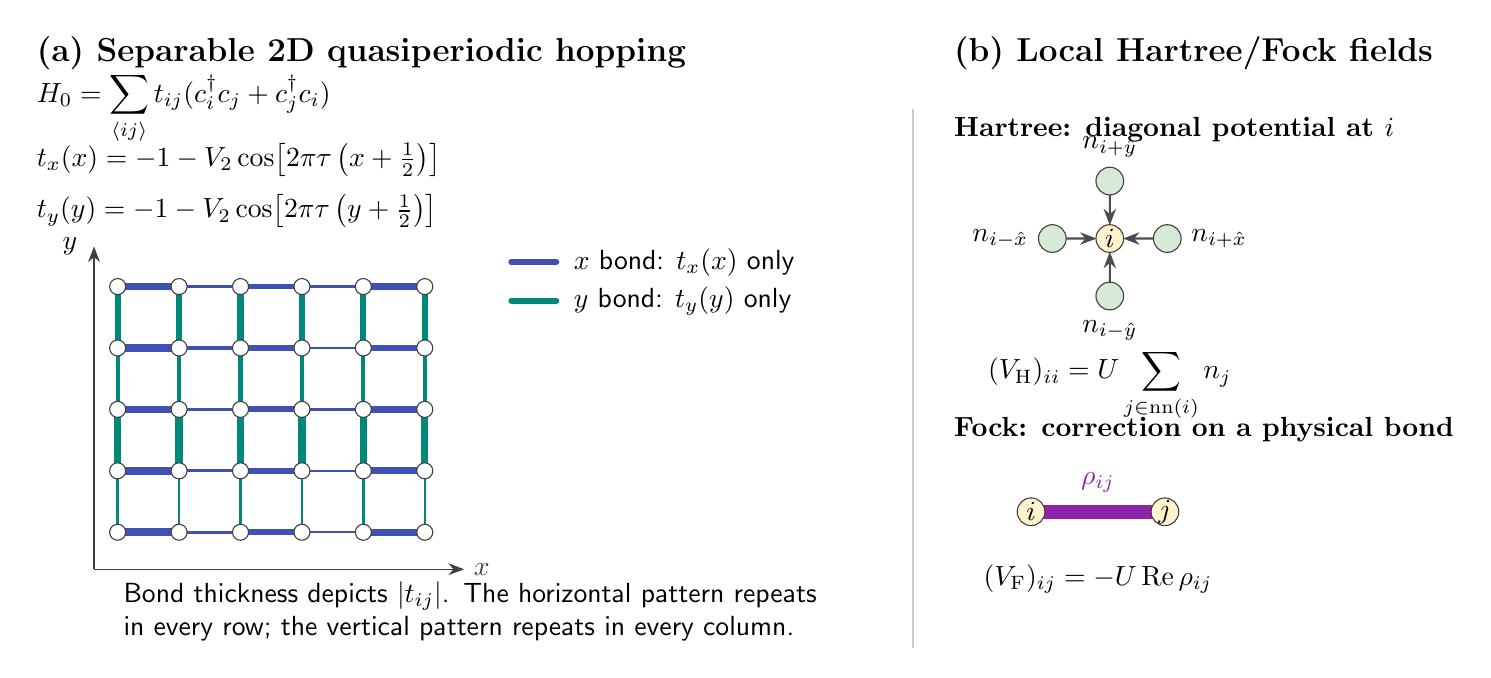
\begin{tikzpicture}[font=\sffamily]

  % Panel (a)
  \node[anchor=west,font=\bfseries\large] at (0,7.8)
    {(a) Separable 2D quasiperiodic hopping};
  \node[anchor=west] at (0,7.1)
    {$\displaystyle H_0=\sum_{\langle ij\rangle}t_{ij}(c_i^\dagger c_j+c_j^\dagger c_i)$};
  \node[anchor=west] at (0,6.45)
    {$\displaystyle t_x(x)=-1-V_2\cos\!\left[2\pi\tau\left(x+\tfrac12\right)\right]$};
  \node[anchor=west] at (0,5.8)
    {$\displaystyle t_y(y)=-1-V_2\cos\!\left[2\pi\tau\left(y+\tfrac12\right)\right]$};

  % lattice locations
  \foreach \x in {0,...,5}
    \foreach \y in {0,...,4}
      \coordinate (a\x\y) at (1.15+\x*.78,1.72+\y*.78);

  % x bonds: thickness varies only by x, hence repeats in every y row
  \foreach \y in {0,...,4} {
    \draw[x bond,line width=2.8pt] (a0\y)--(a1\y);
    \draw[x bond,line width=1.2pt] (a1\y)--(a2\y);
    \draw[x bond,line width=2.1pt] (a2\y)--(a3\y);
    \draw[x bond,line width=.8pt] (a3\y)--(a4\y);
    \draw[x bond,line width=2.5pt] (a4\y)--(a5\y);
  }
  % y bonds: thickness varies only by y, hence repeats in every x column
  \foreach \x in {0,...,5} {
    \draw[y bond,line width=.9pt] (a\x0)--(a\x1);
    \draw[y bond,line width=2.6pt] (a\x1)--(a\x2);
    \draw[y bond,line width=1.5pt] (a\x2)--(a\x3);
    \draw[y bond,line width=2.2pt] (a\x3)--(a\x4);
  }
  \foreach \x in {0,...,5}
    \foreach \y in {0,...,4}
      \node[site] at (a\x\y) {};

  \draw[-{Stealth[length=2mm]},black!75] (.85,1.25)--(5.55,1.25) node[right] {$x$};
  \draw[-{Stealth[length=2mm]},black!75] (.85,1.25)--(.85,5.35);
  \node[anchor=east] at (.76,5.35) {$y$};
  \draw[x bond,line width=2.2pt] (6.15,5.15)--(6.72,5.15);
  \node[anchor=west] at (6.82,5.15) {$x$ bond: $t_x(x)$ only};
  \draw[y bond,line width=2.2pt] (6.15,4.66)--(6.72,4.66);
  \node[anchor=west] at (6.82,4.66) {$y$ bond: $t_y(y)$ only};
  \node[anchor=west,align=left,text width=8.9cm] at (1.1,.72)
    {Bond thickness depicts $|t_{ij}|$. The horizontal pattern repeats in every row; the vertical pattern repeats in every column.};

  % vertical separator
  \draw[black!20,line width=.8pt] (11.25,.25)--(11.25,7.1);

  % Panel (b): Hartree
  \node[anchor=west,font=\bfseries\large] at (11.65,7.8)
    {(b) Local Hartree/Fock fields};
  \node[anchor=west,font=\bfseries] at (11.65,6.83) {Hartree: diagonal potential at $i$};
  \coordinate (hi) at (13.75,5.45);
  \coordinate (hn) at (13.75,6.18);
  \coordinate (hs) at (13.75,4.72);
  \coordinate (hw) at (13.02,5.45);
  \coordinate (he) at (14.48,5.45);
  \foreach \p/\lab in {hn/{i+\hat y},hs/{i-\hat y},hw/{i-\hat x},he/{i+\hat x}}
    \draw[field arrow] (\p)--($(hi)!0.23!(\p)$);
  \node[density site,label=above:$n_{i+\hat y}$] at (hn) {};
  \node[density site,label=below:$n_{i-\hat y}$] at (hs) {};
  \node[density site,label=left:$n_{i-\hat x}$] at (hw) {};
  \node[density site,label=right:$n_{i+\hat x}$] at (he) {};
  \node[selected site] (hcenter) at (hi) {$i$};
  \node[align=center,anchor=north] at (13.75,4.16)
    {$\displaystyle (V_{\mathrm H})_{ii}=U\sum_{j\in\mathrm{nn}(i)}n_j$};

  % Panel (b): Fock
  \node[anchor=west,font=\bfseries] at (11.65,3.03) {Fock: correction on a physical bond};
  \coordinate (fi) at (12.75,1.98);
  \coordinate (fj) at (14.45,1.98);
  \draw[fock,line width=5pt,line cap=round] (fi)--(fj);
  \node[selected site] at (fi) {$i$};
  \node[selected site] at (fj) {$j$};
  \node[fock,fill=white,inner sep=2pt] at (13.6,2.35) {$\rho_{ij}$};
  \node[align=center,anchor=north] at (13.6,1.43)
    {$\displaystyle (V_{\mathrm F})_{ij}=-U\,\mathrm{Re}\,\rho_{ij}$};
\end{tikzpicture}
\end{document}
